\chapter{Application of the multi-objective approach}
\label{chap:ApplicationExamplesNoGUI}

\abstract{In this chapter, the \gls{moo} techniques are tested and applied to different scenarios. A comparison fo the implementation of several linearization techniques is preseted. Then, a well known benchmark problem is tackled with the presented methodology and compared with different tuning methods. Finally, a LiTaO$_3$ Thin Film Deposition Process is used as a prototype for a large dead-time process and tested using a two cost function arrangement.}

\section{Comparison of the methods to obtain the Pareto front}
\label{sec:Comparison}
In order to compare de efficiency of different linearization methods, different test were performed on the normalized process given by:
%
\begin{equation}
\hat{P}(\hat{s}) = \frac{e^{-\tau_0 \hat{s}}}{\hat{s}+1},
\label{eq:NormP}
\end{equation}
%
with values of $\tau_0$ from $0.1$ to $2$. In order to show the results, the simulations presented in this section only contains the case for $\tau_0=0.5$. The other values of $\tau_0$ give similar results.

For this particular case, the controller is supposed to be represented by the transfer function $C(s,\bm{\theta})$ given by \gls{2dof} \gls{pi} controller:
\begin{equation}
u(s) = C_r(s,\bm{\theta}) r(s) - C_y(s,\bm{\theta}) y(s),
\label{eq:2PIControl}
\end{equation}
where $C_r(s,\theta)$ is the reference controller given by the transfer function:
\begin{equation}
C_r(s,\bm{\theta})= K_p \left(\beta + \frac{1}{T_i s} \right),
\label{eq:CrControl}
\end{equation}
%
and $C_y(s,\theta)$ is the feedback controller given by the transfer function:
\begin{equation}
C_y(s,\bm{\theta})=K_p \left(1 + \frac{1}{T_i s} \right),
\label{eq:CyControl}
\end{equation}
%
The parameters $K_p$, $T_i$ and $\beta$ are as usual, the proportional gain, the integral time and the set-point weight, respectively, which can be grouped as a single vector variable denoted by $\bm{\theta}=\left[K_p,T_i,\beta\right]^{T}$.

In %
\begin{figure}[tb]%
	\centering
	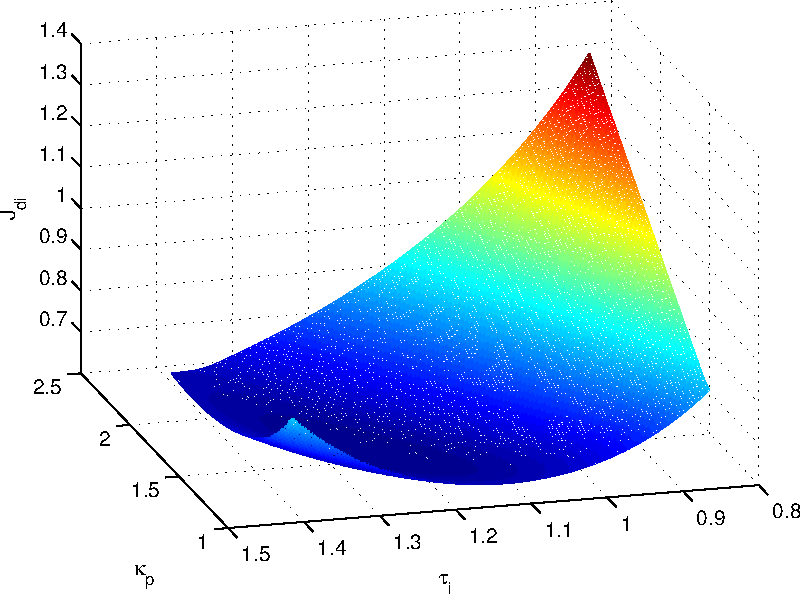
\includegraphics[width=\columnwidth]{RealPareto_t0_05Jdi}%
	\caption{$J_{di}(\hat{\theta})$ function for a value of $\tau_0=0.5$.}%
	\label{fig:RealPareto_t0_05Jdi}%
\end{figure}
%
%
Figure.~\ref{fig:RealPareto_t0_05Jdi}, the cost function $J_{di}(\hat{\theta})$ is plotted as a function of $\kappa_p$ and $\tau_i$, which represent the normalized parameters of the \gls{pi} controller:
\begin{equation}
\begin{array}{c}
\kappa_p \doteq K K_p,\\
\tau_i \doteq \frac{T_i}{T}.
\end{array}
\label{eq:NormContrParam}
\end{equation}

From Figure~\ref{fig:RealPareto_t0_05Jdi}, it can be concluded that the cost function $J_{di}$ is rather convex, and very flat close to its minimal value. The graph in Fig.~\ref{fig:RealPareto_t0_05Jdi} was plotted with ten thousand controller tunings of the controller taking the optimal tuning of $J_{di}(\theta)$ and $J_{do}(\theta)$ as central points. The computation time to obtain this set of data was in the range of hours. In Fig.~\ref{fig:RealParetot0_05}, the complete set of points is plotted in the objective functions plane with the corresponding Pareto front highlighted. The points that represent the Front represents only 3\% of all the points plotted in that figure. If the decision maker is only interested in the  This fact shows the necessity to use some scalarization methods like \gls{nbi} or \gls{nnc} in order to obtain only the front, without the need to compute points that will be dismissed later in the process.
%
\begin{figure}[tb]%
\centering
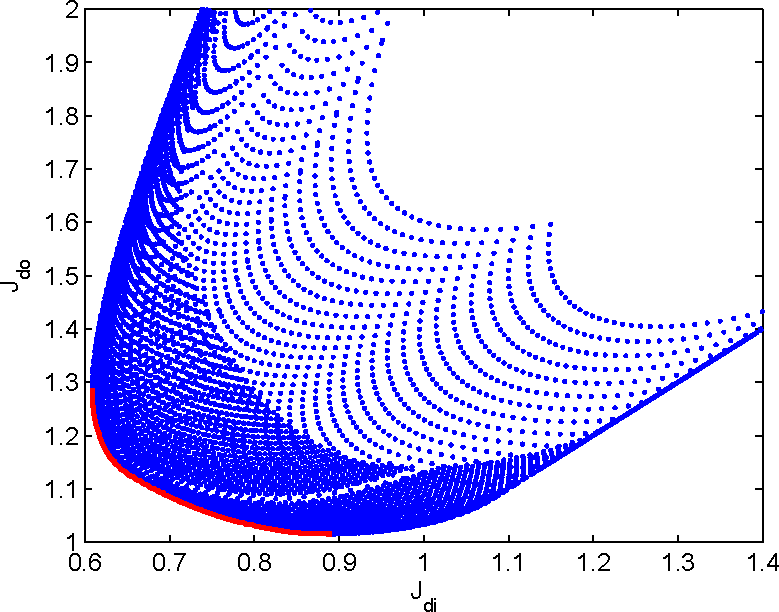
\includegraphics[width=\columnwidth]{RealParetot0_05} %
\caption{Pareto front obtained directly from a ten thousand points data set for \eqref{eq:NormP} with $\tau_0=0.5$.}%
\label{fig:RealParetot0_05}%
\end{figure}

%The Pareto front was obtained with 50 points using the WS, NBI, NNC and LRC methods. 
In Fig.~\ref{fig:ParetoWSt0_05}, the result using WS are presented. The solid line represents the real Pareto front and the points marked with a plus sign correspond to the obtained values. As it can be seen, all the points obtained with the WS method are Pareto optimal, however its distribution is not evenly spaced and are grouped for low values of $J_{di}(\theta)$. This is expected since the shape of the Pareto front does not correspond to the relation needed to obtain a even spaced front with an even spaced parametrization of $\alpha_1$ and $\alpha_2$ as presented in \cite{Das1997}.
%
\begin{figure}[tb]%
\centering
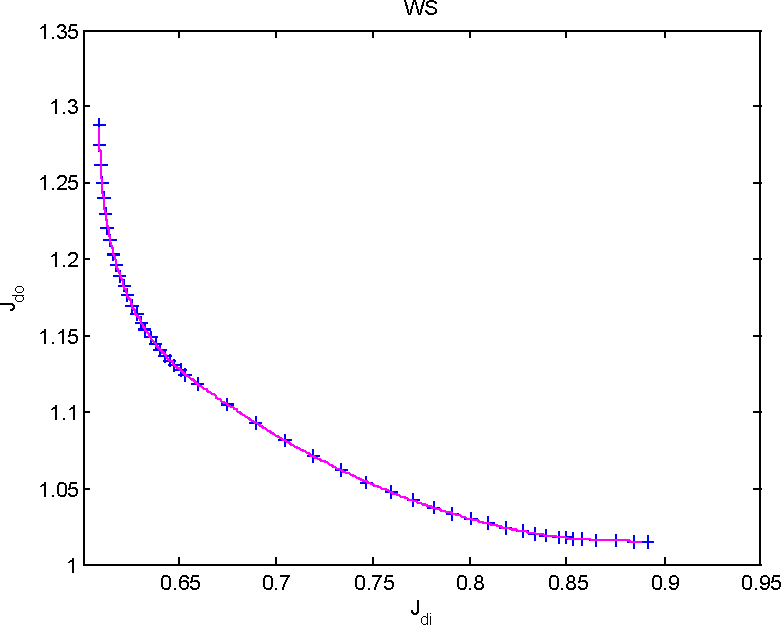
\includegraphics[width=\columnwidth]{ParetoWSt0_05}%
\caption{Pareto front obtained with WS method and $\tau_0=0.5$.}%
\label{fig:ParetoWSt0_05}%
\end{figure}

The result for NBI method is presented in Fig.~\ref{fig:ParetoNBIt0_05}. As it can be seen, the frontier obtained with this method is evenly spaced. It is important to note that the method find different Pareto optimal points than the WS method
%
\begin{figure}[tb]%
\centering
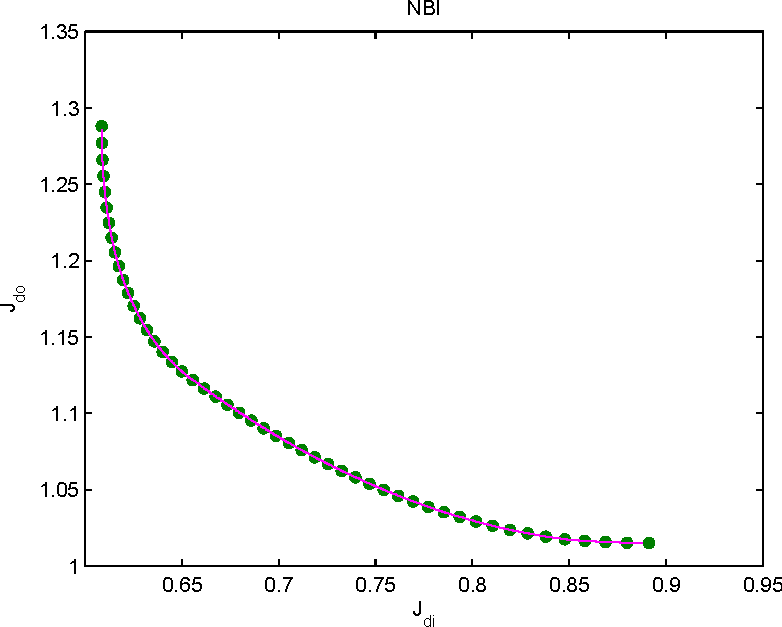
\includegraphics[width=\columnwidth]{ParetoNBIt0_05}%
\caption{Pareto front obtained with NBI method and $\tau_0=0.5$.}%
\label{fig:ParetoNBIt0_05}%
\end{figure}
%

Finally, when the Pareto front is found using the \gls{nnc} method, the points computed are very similar to the ones found with the \gls{nbi} scalarization. The \gls{nnc} case is presented in Fig.~\ref{fig:ParetoNNCt0_05}. 
%
\begin{figure}[tb]%
	\centering
	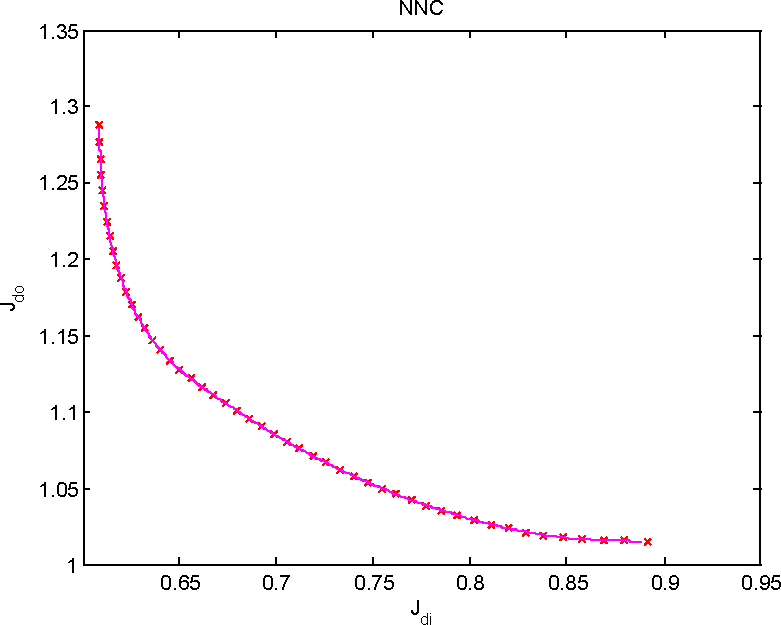
\includegraphics[width=\columnwidth]{ParetoNNCt0_05}%
	\caption{Pareto front obtained with NNC method and $\tau_0=0.5$.}%
	\label{fig:ParetoNNCt0_05}%
\end{figure}
%
Comparing Figure~\ref{fig:ParetoWSt0_05} with Figures~\ref{fig:ParetoNBIt0_05} and \ref{fig:ParetoNNCt0_05}, it is clear that both the \gls{nbi} and \gls{nnc} both are able to find a more accurate approximation of the Pareto front than \gls{ws}. Of course, all the methods are able to find Pareto optimal points, but in order to have a good understanding of the problem, it is important to have a set of point that are representative of the actual behavior of the front. It also is important to note that, the if the actual Pareto front is convex, the results with the \gls{nbi} and \gls{nnc} should be the same. In case of non-convexity, it is possible that the two methods yield to different points in the non-dominated points that should be filtered, following the \gls{nnc} method \cite{Messac2003}.
%
%
%
%The LRC results are found in Fig.~\ref{fig:ParetoLRCt0_05}. In this case, only the $J_{di}(\hat{\theta})$ is evenly spaced, as discussed in Section~\ref{sec:LRC}. It is clear that this new methodology is also capable of finding the Pareto front correctly and with a simpler optimization problem.
%\begin{figure}%
%	\centering
%	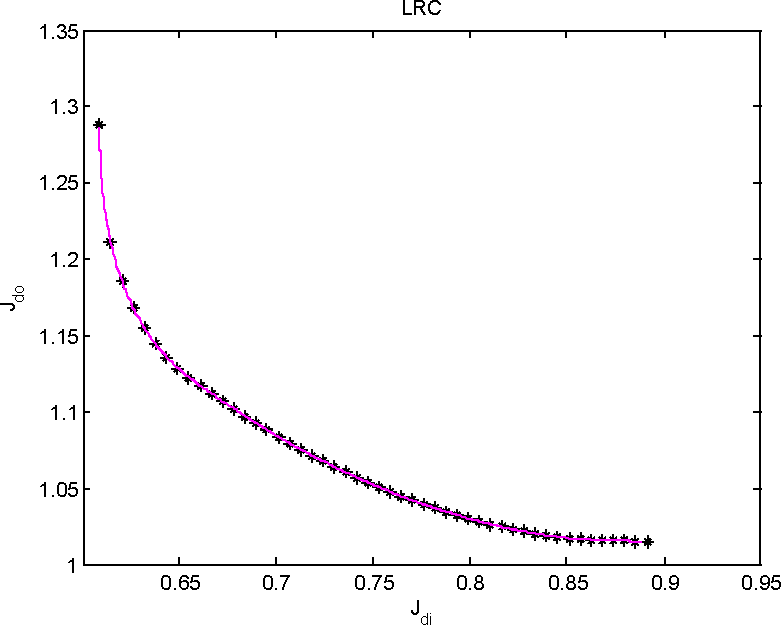
\includegraphics[width=\columnwidth]{ParetoLRCt0_05}%
%	\caption{Pareto front obtained with LRC method and $\tau_0=0.5$. For comparison purposes only, for the LRC method, instead of using $\alpha$ in the abscissa, the value $1-\alpha$ was used instead.}%
%	\label{fig:ParetoLRCt0_05}%
%\end{figure}

In Fig.\ref{fig:KpvsAlpha_t0_05.pdf} the comparison between the results for $\kappa_p$ are presented while the values for $\tau_i$ are shown in Fig.~\ref{fig:TivsAlphat0_05}. 
%
\begin{figure}[tb]
\centering
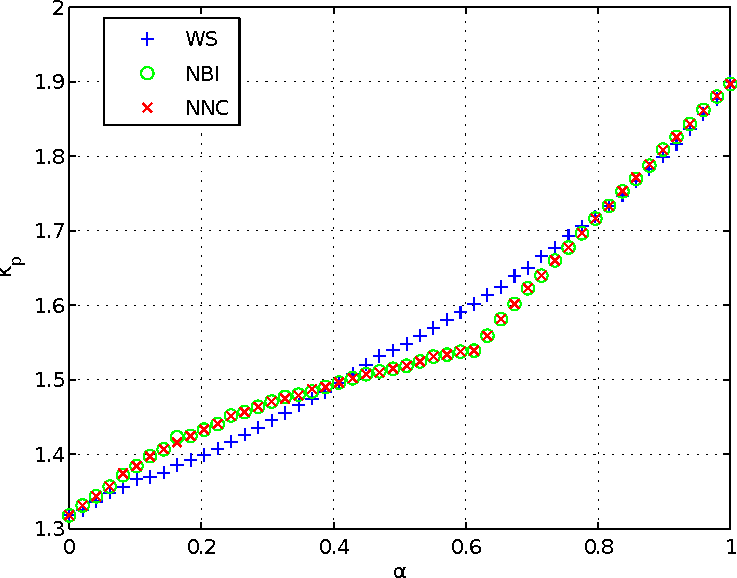
\includegraphics[width=\columnwidth]{KpvsAlpha_t0_05}
\caption{$\kappa_p$ values for all the methods wrt $\alpha$ and with $\tau_0=0.5$.}
\label{fig:KpvsAlpha_t0_05.pdf}
\end{figure}
%%
\begin{figure}[tb]
\centering
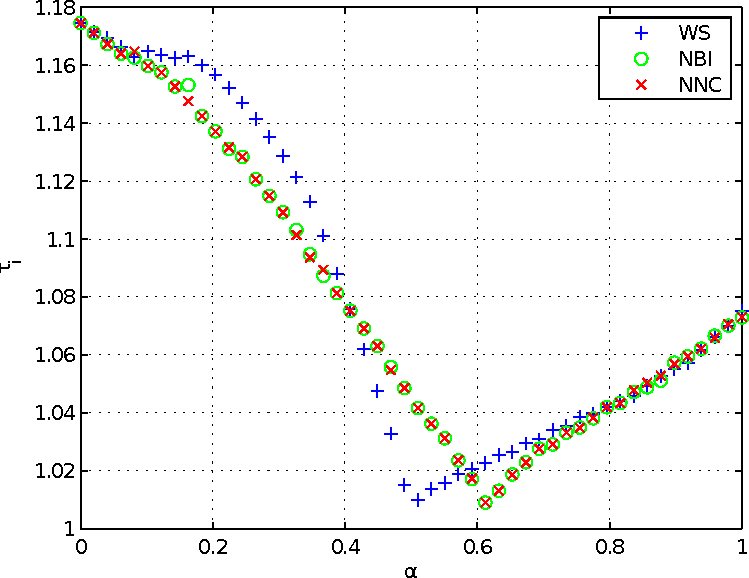
\includegraphics[width=\columnwidth]{TivsAlphat0_05}
\caption{$\tau_i$ values for all the methods wrt $\alpha$ and with $\tau_0=0.5$.}
\label{fig:TivsAlphat0_05}
\end{figure}
%
As it can be seen, \gls{nbi} and \gls{nnc} obtain the exact same points in the Pareto for all values of $\alpha$. However, there are certain differences in the results for $\tau_i$. Since \gls{nbi} depends on a equality constraint, it is more difficult for the optimization algorithm\footnote{For all the methods, the optimization problem was solved using an active-set strategy with a maximum of 1000 iterations and 1000 function evaluations.} to converge to the solution. In fact, for some cases, using the \gls{nbi} methodology lead to more than a thousand function evaluations. Since the maximum was set to one thousand evaluations, for some point the results do not exactly match. However, it is interesting to note that for all three cases, the variation in the values of $\kappa_p$ and $\tau_i$ follows certain pattern. 

The computational performance of the methods has also been considered. Using MATLAB in a PC running Linux with a 3.2.0.2-amd64 kernel and an Intel Core i7 at $1.60$GHz, the results are given in Table~\ref{tab:Results}.
%
\begin{table}%[ht!]
	\caption{Performance comparison for different optimization methods}
	\centering
	\begin{tabular}{ccccccc}
		\toprule
		\multirow{2}{*}{Method} & \multicolumn{2}{c}{Iterations} & \multicolumn{2}{c}{\begin{tabular}{c} Function\\evaluations\end{tabular}} & \multicolumn{2}{c}{\begin{tabular}{c} Computation\\time (s) \end{tabular}}\\
		\cline{2-7}
		& Average & Max & Average & Max & Average & Max \\
		\hline
		WS & $68.82$ & $109$ & $132.34$ & $212$ & $39.11$ & $63.77$\\
		NBI & $30.78$	& $225$ & $142.86$ & $1003$	& $44.88$	& $320.81$\\
		NNC & $41.28$ &	$297$ & $147.02$ & $1002$ & $71.21$	& $486.47$\\
		%LRC	& $12.24$ &	$34$ & $58.56$ & $136$ & $28.45$ & $66.094$\\
		\bottomrule
	\end{tabular}
	\label{tab:Results}
\end{table}
%
This table corresponds to the computation of a fifty point Pareto front for $\tau_0=0.5$. Interestingly, it was found that NNC has lower performance than NBI, for this particular plant. However, it has to be noticed that the NBI reached the evaluation limit in four out of fifty points whereas NNC needed more than a thousand evaluation just once. In all cases the LRC had better performance than the other methods, given its simplicity. Taken the results of the WS method as a reference (since it is the simplest and more intuitive method), the LRC method required $82\%$ less iterations, $56\%$ less function evaluations and $27\%$ less computation time. The NBI and NNC required less iterations than WS but in general, they required more function evaluation ($8\%$ and $11\%$, respectively) and more computation time ($14.74\%$ and $82.05\%$, respectively).

Computing the Pareto front, in total the WS method spent $32.6$ minutes, the NBI $37.4$ minutes, the NNC $59.33$ minutes and the LRC only $23.07$ minutes. It can be seen that the savings in computational load is important. For an offline optimization, the computation time may not be very important, but, if these optimization methods are intended to be used in an online application, the performance and the computation time has to be taken into account.



Therefore, given the present results, it is recommendable to use the NNC method in order to obtain the Pareto front since it gives a better look of the Pareto if the computational load is not an important issue. However, if it is known that the Pareto has a convex shape and it is desirable to have a direct physical meaning associated to the parameter $\alpha$, it is better to use the proposed LRC instead.

Next, the analysis of the results from the control theory point of view are presented. In all cases, the results are as given by the LRC method, since the value of $\alpha$ is directly related to degradation of the response to input disturbance rejection.

%------------------------------------------------------------------------
\subsection{Analysis of the results from the control theory perspective}
\label{sec:Control}
%
When the plant is varied from $\tau_0=0.1$ to $\tau_0=2$ in steps of $0.1$, %the corresponding Pareto fronts are plotted in Fig.~\ref{fig:Paretos_t0_all}. It was expected that for increasing values $\tau_0$, the values of $J_{di}$ and $J_{do}$ also increase because of the inherent delay of the plant which directly affect the IAE.
%\begin{figure}%
%\centering
%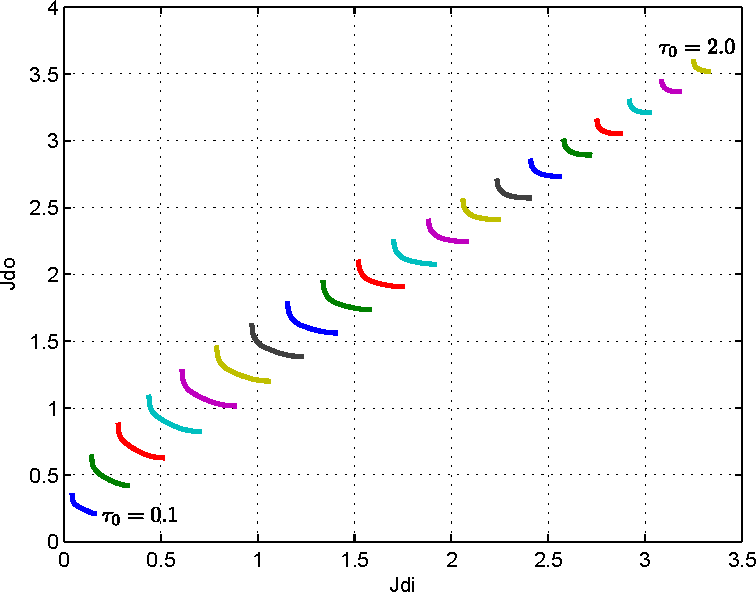
\includegraphics[width=\porcentajefig\columnwidth]{Paretos_t0_all}%
%\caption{Fifty point Pareto fronts varying $\tau_0$.}%
%\label{fig:Paretos_t0_all}%
%\end{figure}
%
it is interesting to analyze the normalized Pareto front for different values of $\tau_0$ as presented in  Fig.~\ref{fig:Paretos_t0_Norm}. %Since the Pareto fronts have different shapes according to $\tau_0$ (see Fig.~\ref{fig:Paretos_t0_all}) it is expected that the normalized versions also vary their shape. However,
It is important to note that, a degradation of nearly $10\%$ in $J_{di}$ leads to an improvement of $50\%$ in $J_{do}$ for all $\tau_0$. In the other hand, if the controller is firstly tuned to optimally reject output disturbances, point $(1,0)$ in the plane, and then is degraded up to $10\%$, the input disturbances rejection is improved almost $40\%$ for $\tau_0 \geq 1.3$. For lower values of $\tau_0$, the same improvement in $J_{di}$ requires a greater degradation in $J_{do}$.
\begin{figure}%
	\centering
	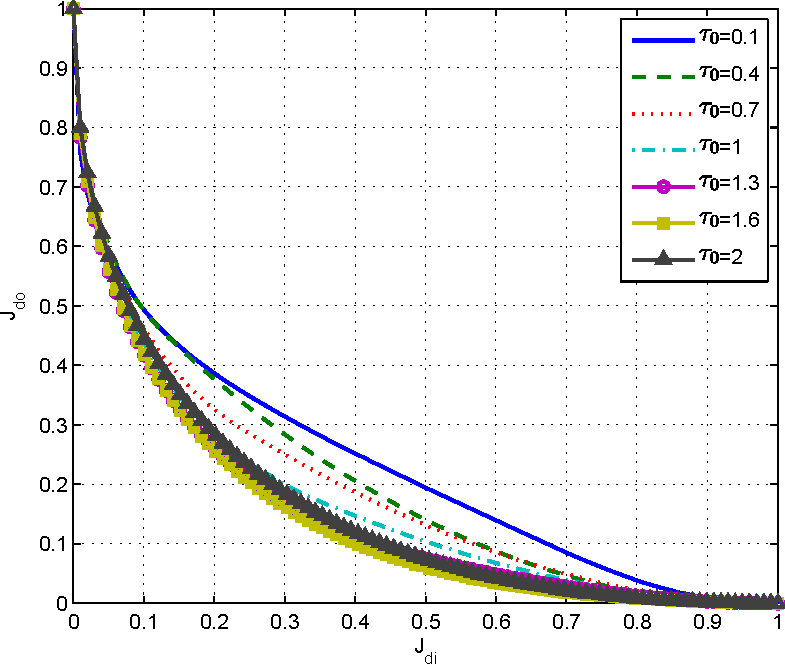
\includegraphics[width=\columnwidth]{Paretos_t0_Norm}%
	\caption{Normalised version of the Pareto front for different values of $\tau_0$.}%
	\label{fig:Paretos_t0_Norm}%
\end{figure}
%
From these results, an important improvement can be achieved in one of the objective functions by degrading a small amount of the other function. The amount of degradation entirely depends on the designer and the characteristics of the plant. However, it is clear that the Pareto front can be considered as a good tool in order to take the decision on how much degradation is necessary (or allowable). 

%Is it possible to identify a single point in the Pareto front that gives the best compromise between these objectives? Although how much degradation is allowed is a subjective decision of the designer, it may be possible to give an alternative. The point that may be a good start is the point in the Pareto front that is closer to the utopia point. This point can be obtained by minimizing
%%
%\begin{equation}
%\min_{\hat{\theta}}{\; \sqrt{\left( \hat{J}_{di}(\hat{\theta})\right) ^2+\left( \hat{J}_{do}(\hat{\theta})\right)^2}}.
%\label{eq:Compr}
%\end{equation}
%%
%The result for $\tau_0=0.5$ is presented in Fig.~\ref{fig:ComprPoint_t0_05}. It is necessary to use the normalized equation as proposed in \eqref{eq:NormalizedJ} in order to give the same importance to both objective functions. 
%%
%\begin{figure}
%\centering
%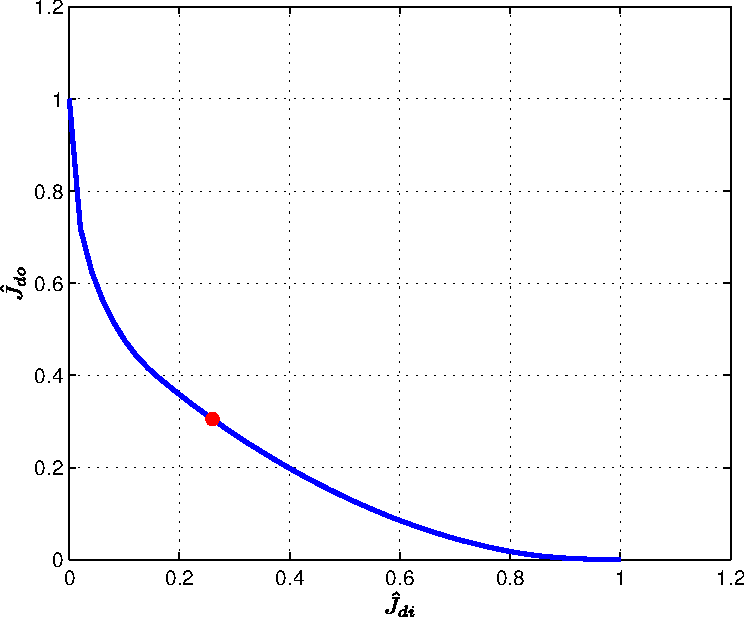
\includegraphics[width=\porcentajefig\columnwidth]{ComprPoint_t0_05}
%\caption{Best compromise in the Pareto front.}
%\label{fig:ComprPoint_t0_05}
%\end{figure}
%%
%As it can be seen, the tuning of the parameters that are closer to the utopia point is the one that produces a degradation of $26\%$ in $\hat{J}_{di}(\hat{\theta})$ and a corresponding $30.52\%$ degradation in $\hat{J}_{do}(\hat{\theta})$. This point may not be suitable for the requirements of the problem at hand, but is a good start point from where the designer can choose the ``best'' (not necessarily the optimal) solution for the particular problem.

%In Fig.~\ref{fig:KpvsAlpha} and \ref{fig:TivsAlpha} the variation of the parameters $\kappa_p$ and $\tau_i$ wrt $\alpha$ for different values of $\tau_0$ are presented. It is interesting to note that the variation in the values of the parameters decrease with higher values of $\tau_0$. If the controller does not allow a precise input of the parameter tuning, it may be possible that the desire point in the Pareto front cannot be achieved for high values of $\tau_0$, since small changes in the tuning produce important changes in the degradation (in percentage). However, it has to be noted in Fig.~\ref{fig:Paretos_t0_all} that the possible change in IAE for both input and output disturbances rejection is smaller for higher values of $\tau_0$ than for lower values. The relationship between $\kappa_p$ and $\tau_i$ is presented in Fig.~\ref{fig:TivsKp}. The possible range of values is also smaller for higher values of $\tau_0$. 
%\begin{figure}%
%\centering
%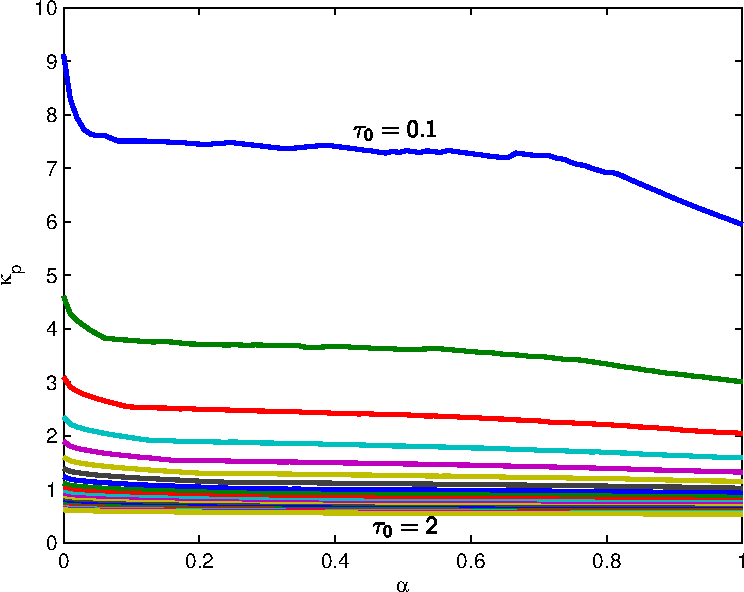
\includegraphics[width=\porcentajefig\columnwidth]{KpvsAlpha}%
%\caption{Variation of $\kappa_p$ wrt $\alpha$ and $\tau_0=0.5$.}%
%\label{fig:KpvsAlpha}%
%\end{figure}
%%
%\begin{figure}%
%\centering
%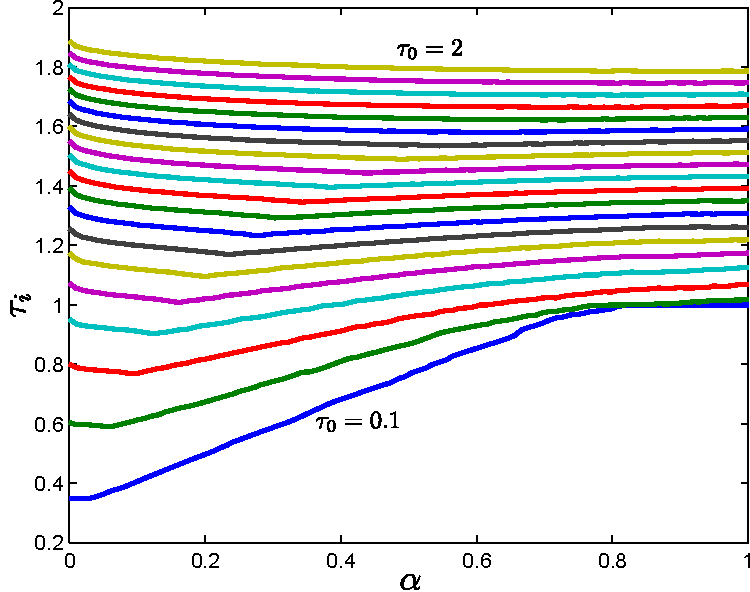
\includegraphics[width=\porcentajefig\columnwidth]{TivsAlpha}%
%\caption{Variation of $\tau_i$ wrt $\alpha$ and $\tau_0=0.5$.}%
%\label{fig:TivsAlpha}%
%\end{figure}
%%
%\begin{figure}%
%\centering
%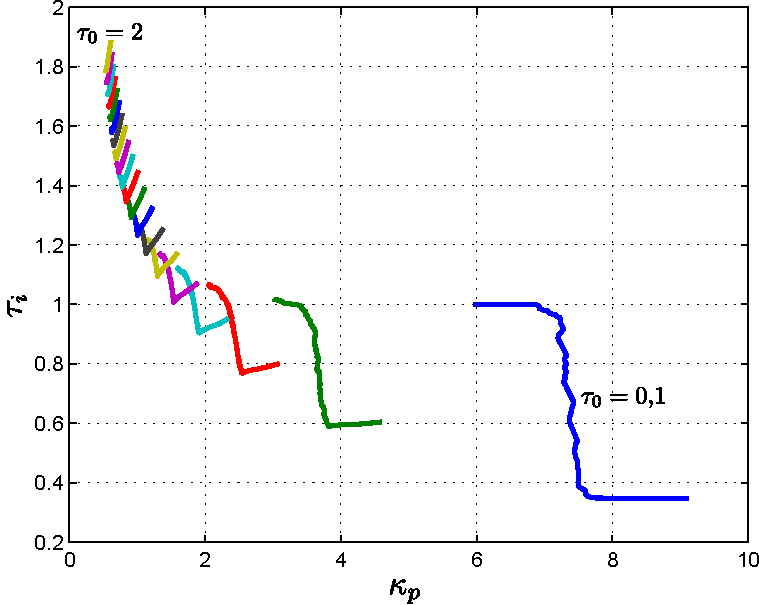
\includegraphics[width=\porcentajefig\columnwidth]{TivsKp}%
%\caption{$\tau_i$ vs $\kappa_p$ for different values of $\tau_0$.}%
%\label{fig:TivsKp}%
%\end{figure}
%%

In order to check the relationship between different tuning methodologies and the Pareto front, the objective functions were computed for different well known tuning methodologies (see \cite{ODwyer2000,Astrom1995,Murril1967,Rovira1969,Grimholt2012, Smith1985, Ziegler1942}). The results are presented in Fig.~\ref{fig:PIMethods}. 
\begin{figure}%
	\centering
	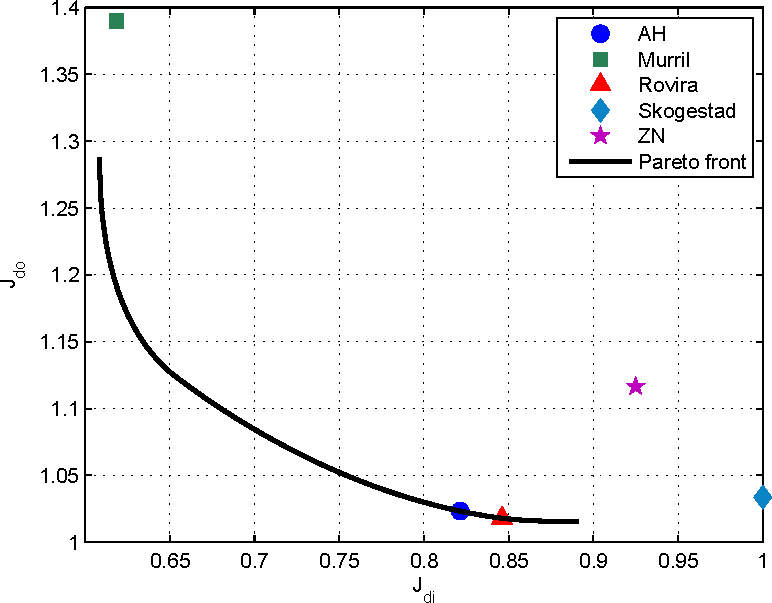
\includegraphics[width=\columnwidth]{PIMethods}%
	\caption{Comparison of several tuning methods within the Pareto front for $\tau_0=0.5$.}%
	\label{fig:PIMethods}%
\end{figure}
%
The tuning of Murril~\cite{Murril1967} was intended to minimize IAE for input disturbances. This explains the fact that the value of $J_{di}$ is almost minimal. From a Pareto perspective the results for $J_{do}$ could have been slightly improved.%However it has to be take into account that the method was proposed more than forty years ago when the computing power was not as powerful as nowadays.

The tuning of Rovira~\cite{Rovira1969} minimizes the servo response. For a one degree of freedom controller, minimizing the servo response is exactly the same as minimizing the output disturbance rejection for a two degrees of freedom controller. Therefore, it is not a surprise that the tuning point is located at the right hand side of the Pareto front. Special mention has to be given to the tuning of {\AA}ström and Hägglund \cite{Astrom1995} (AH in the figure), because it ended to be Pareto optimal, but was better suited for servo response. The case of Skogestad \cite{Grimholt2012} is interesting because it is almost optimal in the $J_{do}$ sense, but due to its consideration of robustness, its far from the Pareto front. The Ziegler and Nichols tuning \cite{Ziegler1942} (ZN in the figure) is included here for comparison purposes only.

It has to be noticed that the results obtained in this work using the Pareto front concept do not consider the robustness of the closed-loop system. In Fig.~\ref{fig:MsAlpha}, the obtained maximum sensitivity is presented as a function of $\alpha$ for different values of $\tau_0$. As it is expected, the robustness of the controlled system is not adequate for these optimal settings (almost for all cases, the value of $M_S$ is greater than 2). For a degradation of $J_{di}$ greater than $0.9$, the sensitivity function is near 2, but the performance of the input disturbance rejection has been almost lost (from the Pareto front point of view).
\begin{figure}%
	\centering
	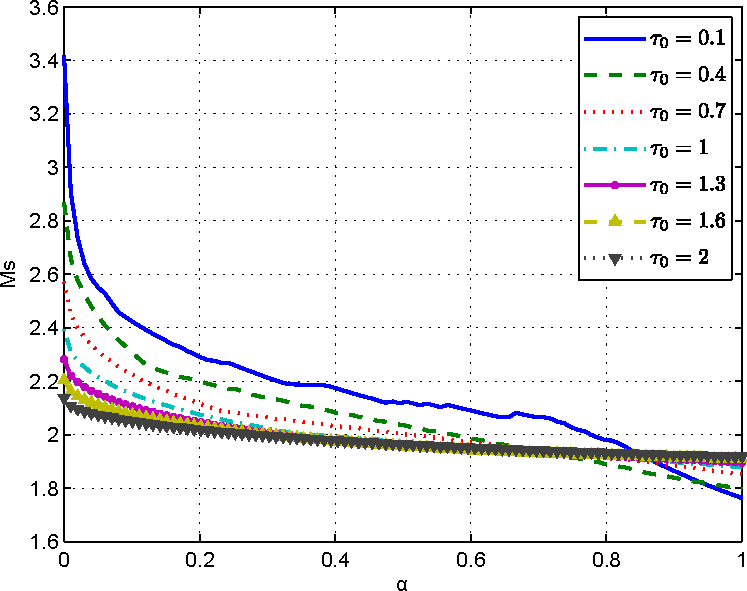
\includegraphics[width=\columnwidth]{MsAlpha}% %\porcentajefig
	\caption{Sensitivity function wrt $\alpha$, varying $\tau_0$.}%
	\label{fig:MsAlpha}%
\end{figure}
%
Nevertheless, it is easy to deal with the robustness, since it can be considered to be a (non-linear) constraint in the optimization problem. That is, the feasible region is shrink to the cases in which the robustness is fulfilled.
%As an example, consider the case of $\tau_0=0.5$ presented in Fig.~\ref{fig:Pareto10000MS16}. When the case for $M_S\leq 1.6$ is considered, the feasible region is shrink considerably. In this case, the Pareto front for the optimal tuning is outside the new feasible region and therefore, a completely different Pareto front would be obtained when the optimization methods are run considering this new constraint. Depending of the desired value of $M_S$ and the given value of $\tau_0$, it may be possible that the optimal frontier also satisfy the robustness constraint.
%
%\begin{figure}%
%\centering
%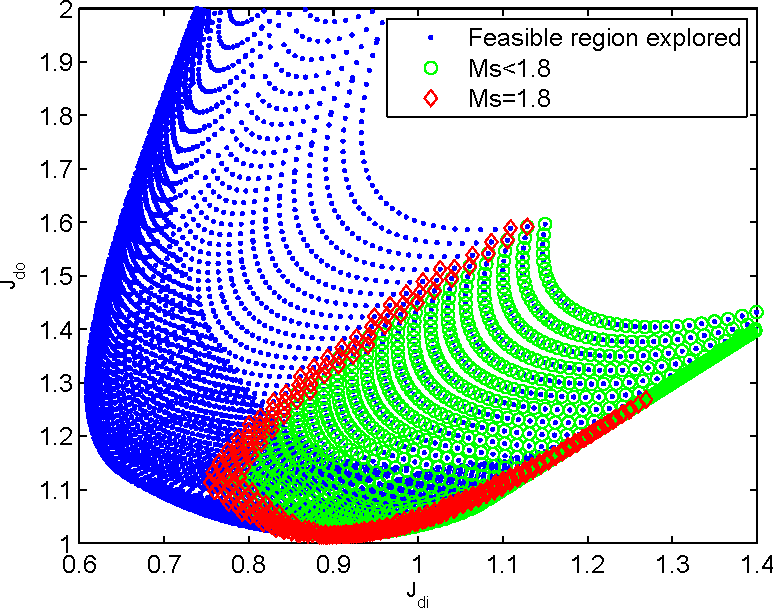
\includegraphics[width=\porcentajefig\columnwidth]{Pareto10000MS16}%
%\caption{Complete feasible region for $\tau_0=0.5$ and the subregion where $M_S \leq 1.8$.}%
%\label{fig:Pareto10000MS16}%
%\end{figure}
%
Therefore, since the robustness can be considered just as a constraint in the optimization problem, a tuning methodology that considers both multi-objective optimality and robustness can be obtained using the Pareto front framework.
%
%---------------------------------------------------------------------------------------
%---------------------------------------------------------------------------------------
%
%\section{High order benchmark plant}
%\label{sec:Bechmark}
%First the \gls{ennc} method is going to be tested in high order benchmark plant \citep{Astroem2000}. The model of the plant is given by a fourth order transfer function:
%\begin{equation}
%P(s) = \frac{1}{\prod_{n=0}^{n=3}(0.5^n s+1)}.
%\label{eq:benchmarkTF}
%\end{equation}
%
%The first step is to obtain a low order model that is able to reflect the main dynamics of the plant. In general, the tuning of \gls{pid} controllers starts with a first or second order model \citep{Alfaro2006}. In this particular case, using a step change as the input signal, the low order model that can be found from this experiment is given by:
%%
%\begin{equation}
%F(s)=\frac{e^{-0.297s}}{(0.9477s+1)(0.6346s+1)},
%\label{eq:BenchTFfit}
%\end{equation}
%%
%alternatively, if it is supposed that the ``real'' model of the plant is known, an order reduction procedure, for example, the half-rule method may be used \citep{Skogestad2003}. The comparison between the high order model and the reduced order model in the time domain is presented in %
%\begin{figure}[tb]
%	\centering
%	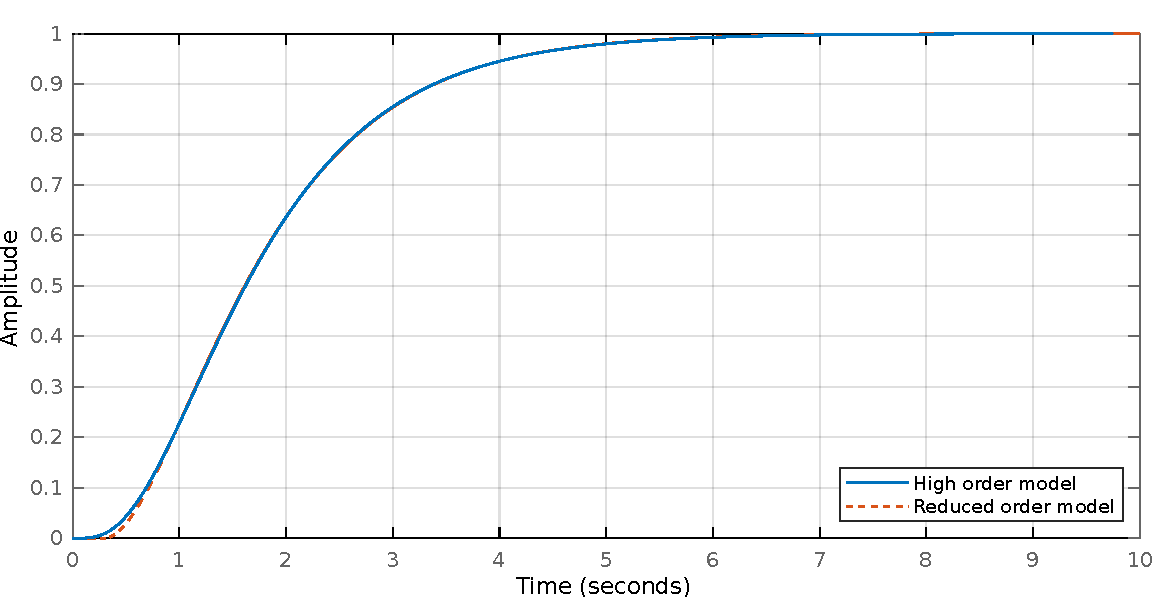
\includegraphics[width=0.9\columnwidth]{Ch7CompRespBench}
%	\caption{Comparison between the high and reduced order models.}
%	\label{fig:Ch7CompRespBench}
%\end{figure}
%%
%Figure~\ref{fig:Ch7CompRespBench}. As it can be seen, the model represent accurately the dynamics of the original plant and therefore is considered to be a good approximation of the original model.
%
%The next step is to find the Pareto front for this particular plant. The followed methodology was as presented in Chapter~\ref{chap:PIDMOOP}. For this particular case, only $J_{di}$ and $J_r$ where considered as the cost functions with a \gls{2dof} \gls{pid} controller. In Figure~\ref{fig:paretomodelo}, the obtained Pareto front is presented. 
%%^
%\begin{figure}[tb]%
%	\centering
%	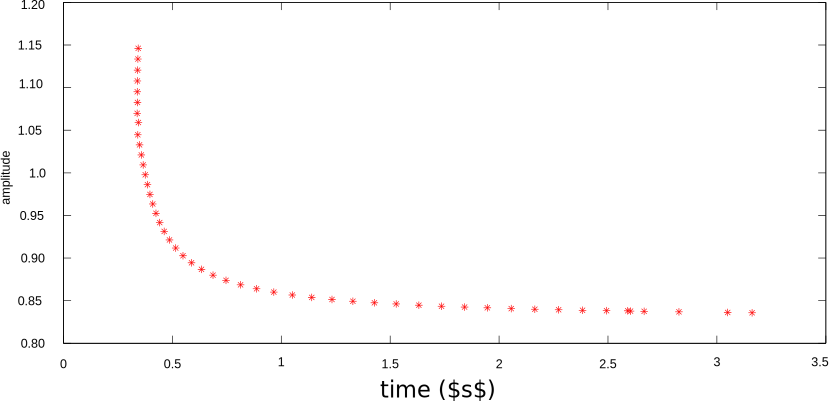
\includegraphics[width=0.9\columnwidth]{paretomodelo}%
%	\caption{The Pareto front for the benchmark process.}%
%	\label{fig:paretomodelo}%
%\end{figure}
%
%The curve has a typical form, with a high slope for low values of $J_{di}$ and an almost flat slope for higher values. This shape has a particular physical meaning: to improve the response of the $J_{di}$ cost function, the $J_{r}$ value has to be augmented (worsening the servo response), however the degradation is not as much as the improvement in the $J_{di}$ function. This is a clear example of one of the many advantages of using a multi-objective framework for controller tuning and the main reason why is the chosen framework in this book, it gives the decision taker more tools to select the more appropriate tuning for the controllers.
%
%In order to compare the response of the optimal controllers, the tuning for the anchor points are presented along the resposes of the ART$_2$ method \citep{Vilanova2011} and the uSORT$_2$ method\citep{Alfaro2012a}, in order to compare the performance of the closed loop response. It is important to clarify that these two tuning are just the extreme points of the Pareto front, thanks to the ENNC method and that there is a practically and infinite amount of possible parameter tuning to select. The obtained parameters are listed in %
%%
%%parámetros del controlador
%\begin{table}[tb]
%	\caption{PID controller parameters using two degrees of freedom.}
%	\centering
%	\begin{tabular}{@{}*{5}{c}@{}}
%		\toprule
%		Tuning              &$K_c$       &$T_i$      &$T_d$     & $\beta$ 	\\
%		\midrule              
%		optimum $J_{di}$     &$3.3750$   & $1.0812$  &$0.3095$  &$0.5466$   \\
%		optimum $J_{r}$      &$3.0572$   & $8.4419$  &$0.3986$  &$1.2329$   \\
%		$ART_2$             &$3.3657$   & $1.7636$  &$0.4884$  &$0.2971$   \\
%		$uSORT_2$           &$3.1708$   & $0.8997$  &$0.3945$  &$0.4731$   \\	
%		%
%		\bottomrule				
%	\end{tabular}
%	\label{tab:parametroscontrolador}
%\end{table}
%%
%Table~\ref{tab:parametroscontrolador} for reference. It is important to note that in all cases, the Maximum Sensibility was set to be around $M_s = 2.0$ to ensure a minimum level of robustness.
%
%In Figure~\ref{fig:Ch7cambioreferencia}, the closed-loop responses of all the four controllers are presented for the case of a step change in the setpoint. it was found that precisely the controller in the anchor point of the Pareto front that give the minimum value of $J_r$ is in fact the one that give the best result of all the controllers. However, it has to be noticed that both ART$_2$ and uSORT methods are intended for regulator response mainly, and theredore, it was not expected to have a low $J_r$. The obtained values are given in Table~\ref{tab:IAEref} where both the \gls{iae} and \gls{ms} are presented. 
%
%On the other hand, the optimal controllers in the regulator mode are presented in Figure~\ref{fig:cambiodi}. Again, as expected, the controller in the anchor point that has the lowest value of $J_{di}$, is the one with the fastest response. Also, it is clear that the other anchor point (the one with the lowest value of $J_r$) has the worst response for disturbance rejection as it was expected. In table \ref{tab:IAEdi}, the corresponding values of IAE for the curves in Figure~\ref{fig:cambiodi} are presented.
%
%The optimal controller for disturbance rejection is presented in figure \ref{fig:cambiodi}. Again, the tuning given by the ENNC method is the fastest response to reach the desired value. As it can be seen, the ART$_2$ and the uSORT$_{2}$ methods fall between these two optimal responses. However, it does not necessarily means that these methods are optimal because they could be dominated by other controllers that are exactly in the front. Only the tuning found with the ENNC method can be considered to be Pareto optimal using the \gls{iae} as the metric. In Table~\ref{tab:IAEdi}, the IAE values of the responses presented in Figure~\ref{fig:cambiodi} are stated, and again the controller that achieves the lower error value is the one that correspond to the anchor point.
%%CAMBIO EN VALOR REFERENCIA
%\begin{figure}[tb]%
%	\centering
%	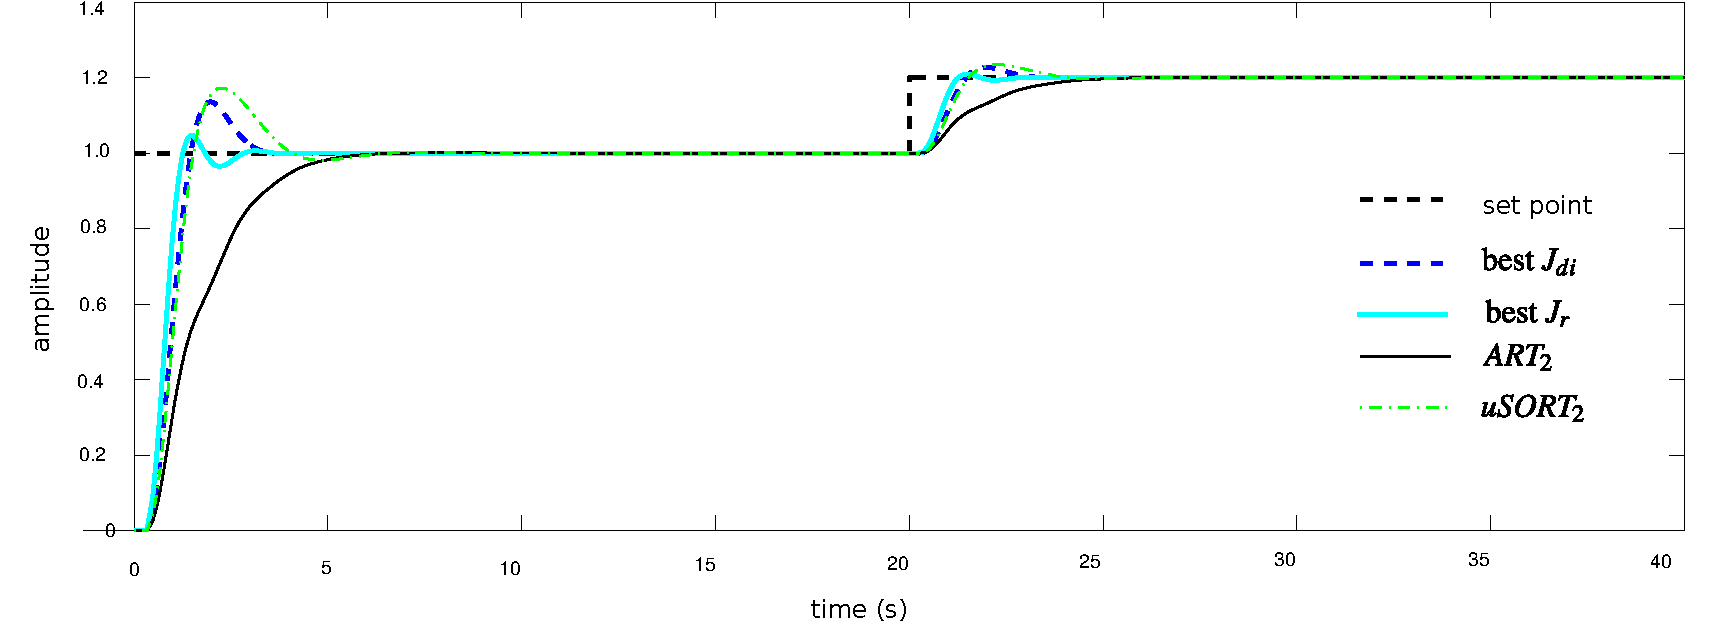
\includegraphics[width=\columnwidth]{Ch7cambioreferencia}%
%	\caption{Optimal response of the control system $J_r$}%
%	\label{fig:Ch7cambioreferencia}%
%\end{figure}
%%
%%CAMBIO EN PERTURBACIÓN
%\begin{figure}[tb]%
%	\centering
%	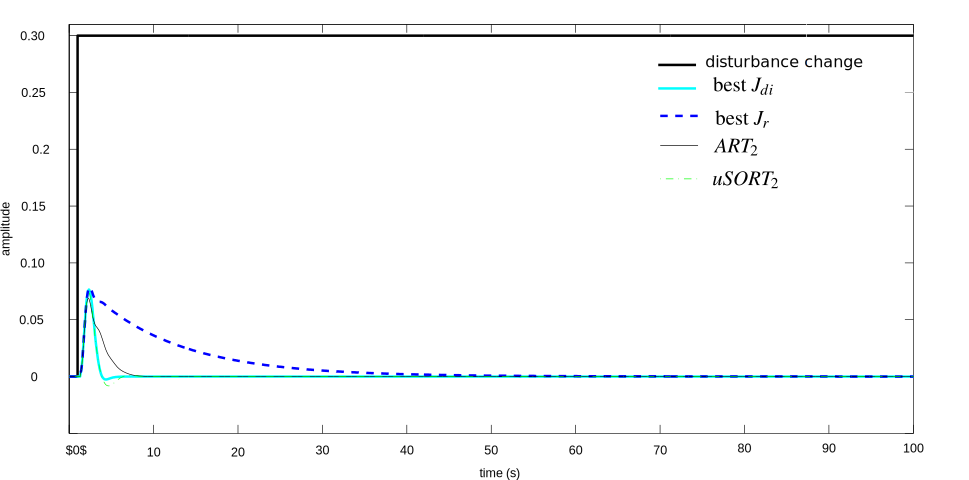
\includegraphics[width=\columnwidth]{cambiodi}%
%	\caption{Optimal response of the control system $J_{di}$}%
%	\label{fig:cambiodi}%
%\end{figure}
%%
%%IAE ante cambio en valor de referencia
%\begin{table}[tb]
%	\caption{Servo response for the benchmark system.}
%	\centering
%	\begin{tabular}{@{}*{3}{c}@{}}
%		\toprule
%		Tuning             &IAE        &$M_s$   \\
%		\midrule              
%		optimum $J_{r}$     &$1.004$   & $2$    \\
%		optimum $J_{di}$    &$1.297$   & $2$    \\
%		$uSORT_2$          &$1.522$   & $2$    \\
%		$ART_2$          &$2.121$   & $2$    \\	
%		\bottomrule				
%	\end{tabular}
%	\label{tab:IAEref}
%\end{table}
%%
%%IAE ante cambio en perturbación
%\begin{table}[tb]
%	\caption{Regulator response for the benchmark system.}
%	\centering
%	\begin{tabular}{@{}*{3}{c}@{}}
%		\toprule
%		Tuning            &IAE        &$M_s$   \\
%		\midrule              
%		optimum $J_{di}$   &$0.1017$   & $2$    \\
%		$uSORT_2$          &$0.1095$   & $2$    \\
%		$ART_2$            &$0.1574$    & $2$    \\	
%		optimum $J_{r}$    &$0.8283$   & $2$    \\
%		\bottomrule				
%	\end{tabular}
%	\label{tab:IAEdi}
%\end{table}
%
%It is important to note that in these figures, only two possible points (in fact, the two extreme cases) were considered, but in reality, there are much more options to select for intermediate values of the parameters between these two cases. It has to be noticed that the second order overdamped model is well suited to approximate high order models. Therefore, having done the computation for this particular model as presented in Section~\ref{sec:SolMOOP} allows to tackle almost any real-case of overdamped plants that can be found in the industry. The tool that was presented in Section~\ref{sec:DatabaseMOOP} is used in Section~\ref{sec:Description} with a more realistic industrial case.
%%-----------------------------------------------------------------------------------------------------------------------------------
%\section{LiTaO$_3$ Thin Film Deposition Process}
%\label{sec:LiTAO3}
%Temperature control is a very important factor in the deposition process of lithium tantalate (LiTaO$_3$) by means of metal organic chemical vapor deposition (MOCVD) \citep{Zhang2004}.
%
%The dynamics of the reactor chamber are characterized by a large lag and time-delay. It is important for the quality of the final product, that the controller follow a predefined temperature profile accurately (servo control) while been able to reject other disturbances (regulatory control).
%
%The model of the MOCVD chamber can be given by:
%\begin{equation}
%G(s) = \frac{K e^{-L s}}{T s+1},
%\label{eq:GsLita}
%\end{equation}
%%
%where the gain $K = 3.2$, the time constant $T = 200$~s and the time-delay $L = 150$~s.
%
%For this case, a two function MOOP is considered with $J_{di}$ and $J_{r}$ as cost functions and a robustness restriction of $M_S = 2.0$. When solving the optimization using the ENNC method, the obtained Pareto front is as given in %
%\begin{figure}[tb]
%	\centering
%	\begin{tikzpicture}
%	\begin{axis}[
%	xlabel = $J_{di}$,
%	ylabel = $J_{r}$,
%	grid = major,
%	width=0.7\columnwidth,
%	xtick={0.7,0.75,...,1.2},
%	ytick={1.2,1.22,...,1.5},
%	]
%	\addplot[mark=none, line width=2pt,] table[x=Jdi, y=Jr]{./tablas/Pareto_LiTa_ms2.dat};
%	\end{axis}
%	\end{tikzpicture}
%	\caption{Pareto front for the LiTaO$_3$ thin film deposition process.}
%	\label{fig:LitaPareto}
%\end{figure}
%%
%figure~\ref{fig:LitaPareto}.
%
%Again, the Pareto front let the decision maker to choose between multiple possible solutions. In this particular case, taking the anchor point for minimum value of $J_{di}$ from Figure~\ref{fig:LitaPareto}, it can be seen that, from this point, if $J_{di}$ is degraded by $1.8\%$, it means an improvement of $4.37\%$ for $J_{r}$. This information could only be possible if the Pareto is available is some way, either as a graph or as a set of raw data.
%
%In order to help the control engineer to understand the tuning of the controller, it could be useful to plot the variation of the controller parameters as a function of the degradation of one of the cost functions. Given that the LiTaO$_3$ Thin Film Deposition Process requires to follow a given temperature profile, the control engineer may surely consider $J_r$ as the main function.
%%
%\begin{figure}[tb]
%	\centering
%	\subfloat[$K_p$ variation for the LiTaO$_3$ thin film deposition process as a function of $J_r$ degradation.]{
%	\begin{tikzpicture}
%	\begin{axis}[
%	label style={font=\scriptsize},
%	tick label style={font=\scriptsize},
%	xlabel = $m$ (\%),
%	ylabel = $K_p$,
%	grid = major,
%	width=0.45\columnwidth,
%	%scaled x ticks={real:0.01},
%	%xtick scale label code/.code={},
%	xtick={0,0.2,...,1.2},
%	scaled x ticks={real:0.01},
%	xtick scale label code/.code={},
%	ytick={0.41,0.412,...,0.44},
%	y tick label style={
%		/pgf/number format/.cd,
%		fixed,
%		fixed zerofill,
%		precision=3,
%		/tikz/.cd
%	}
%	]
%	\addplot[mark=none, line width=1pt,color=brown] table[x=Jrn, y=Kp]{./tablas/Pareto_LiTa_ms2.dat};
%	\end{axis}
%	\end{tikzpicture}
%	\label{fig:LitaParetoKp}}\qquad
%	%
%	\subfloat[$T_i$ variation for the LiTaO$_3$ thin film deposition process as a function of $J_r$ degradation.]{
%		\begin{tikzpicture}
%		\begin{axis}[
%		label style={font=\scriptsize},
%		tick label style={font=\scriptsize},
%		xlabel = $m$ (\%),
%		ylabel = $T_i$,
%		grid = major,
%		width=0.45\columnwidth,
%		xtick={0,0.2,...,1.2},
%		scaled x ticks={real:0.01},
%		xtick scale label code/.code={},
%		%xtick={0,0.1,...,1},
%		ytick={200,220,...,320},
%		]
%		\addplot[mark=none, line width=1pt,color = blue] table[x=Jrn, y=Ti]{./tablas/Pareto_LiTa_ms2.dat};
%		\end{axis}
%		\end{tikzpicture}
%		\label{fig:LitaParetoTi}
%		}\\
%	%
%	\subfloat[$T_d$ variation for the LiTaO$_3$ thin film deposition process as a function of $J_r$ degradation.]{
%		\begin{tikzpicture}
%		\begin{axis}[
%		label style={font=\scriptsize},
%		tick label style={font=\scriptsize},
%		xlabel = $m$ (\%),
%		ylabel = $T_d$,
%		grid = major,
%		width=0.45\columnwidth,
%		xtick={0,0.2,...,1.2},
%		scaled x ticks={real:0.01},
%		xtick scale label code/.code={},
%		%xtick={0,0.1,...,1},
%		ytick={40,41,...,55},
%		]
%		\addplot[mark=none, line width=1pt,color = red] table[x=Jrn, y=Td]{./tablas/Pareto_LiTa_ms2.dat};
%		\end{axis}
%		\end{tikzpicture}
%		\label{fig:LitaParetoTd}
%		}\qquad
%	%
%	\subfloat[$\beta$ variation for the LiTaO$_3$ thin film deposition process as a function of $J_r$ degradation.]{
%		\begin{tikzpicture}
%		\begin{axis}[
%		label style={font=\scriptsize},
%		tick label style={font=\scriptsize},
%		xlabel = $m$ (\%),
%		ylabel = $\beta$,
%		grid = major,
%		width=0.45\columnwidth,
%		xtick={0,0.2,...,1.2},
%		scaled x ticks={real:0.01},
%		xtick scale label code/.code={},
%		%xtick={0,0.1,...,1},
%		ytick={0.65,0.7,...,1.05},
%		]
%		\addplot[mark=none, line width=1pt,color = olive] table[x=Jrn, y=beta]{./tablas/Pareto_LiTa_ms2.dat};
%		\end{axis}
%		\end{tikzpicture}
%		\label{fig:LitaParetoBeta}	
%	}
%	%
%	\caption{Variation of the parameters vs $J_r$ for the  LiTaO$_3$ thin film deposition process.}
%	\label{fig:LitaParetoParam}
%\end{figure}
%%
%
%In Figure~\ref{fig:LitaParetoParam} the values of all the controller parameters are plotted against $m$, where $m$ is defined as the normalized degradation of $J_{r}$ ($m=0$ represents the anchor point where $J_r$ has its lowest value). Looking the behaviour of $K_p$ in Figure~\ref{fig:LitaParetoKp}, it is clear that the value of $K_p$ is kept fairly constant for all values of $m$. This almost negligible variation may be associated to the fact that, for all controller tunings, the maximum sensitivity is set at $M_S = 2$. When this constraint is not taken into account, the value of $K_p$ may have large variations as in the example in Section~\ref{sec:CSTH}.
%
%For the case of the integral time $T_i$, the behavior of this parameter is plotted in Figure~\ref{fig:LitaParetoTi}. Note that, contrary to the case of $K_p$, the variation is highly dependent of $J_r$ and fairly smooth, which is desirable if the interest is to find a tuning rule. However, for the derivative time $T_d$ in Figure~\ref{fig:LitaParetoTd}, it can be seen that the variation is important but the behavior is not as near as smooth as in the case of $T_i$. Finally and the setpoint weight factor $\beta$, also has a piece-wise behavior with respect to $J_r$ and also the variation of its value is important. Nevertheless, once computed the corresponding tunings of all the controllers of the Pareto, is just to pick and decide which one is more appropriate for the task.
%
%The response of the controlled system to a setpoint step change is presented in %
%%
%\begin{figure}[tb]
%	\centering
%	\begin{tikzpicture}
%	\begin{axis}[
%	label style={font=\scriptsize},
%	tick label style={font=\scriptsize},
%	xlabel = time~(s),
%	ylabel = output,
%	legend cell align=left,
%	legend style = {legend pos = south east, font=\scriptsize},%{at={(1,0.05)}, anchor=south east},%
%	grid = major,
%	width=\columnwidth,
%	%scaled x ticks={real:0.01},
%	%xtick scale label code/.code={},
%	xtick={0,200,...,1600},
%	%ytick={41,42,...,52},
%	]
%	\addplot[mark=none, color=red] table[x=time, y=r]{./tablas/TestServo.dat};
%	\addplot[mark=none,dashed, color=blue] table[x=time, y=yservo]{./tablas/TestServo.dat};
%	\addplot[mark=none,densely dashdotdotted, color=olive] table[x=time, y=yreg]{./tablas/TestServo.dat};
%	\addplot[mark=none,dashdotted, color=magenta] table[x=time, y=yusort]{./tablas/TestServo.dat};
%	\legend{Reference,$m=0\%$ (IAE=$244.66$), $m=100\%$ (IAE=$285.64$),uSORT$_2$ (IAE=$304.39$)}
%	\end{axis}
%	\end{tikzpicture}
%	\caption{Servo response of the LiTaO$_3$ thin film deposition process with tree different tuning.}
%	\label{fig:LitaServo}
%\end{figure}
%%
%figure~\ref{fig:LitaServo} and for a step signal in the input disturbance in %
%%
%\begin{figure}[tb]
%	\centering
%	\begin{tikzpicture}
%	\begin{axis}[
%	label style={font=\scriptsize},
%	tick label style={font=\scriptsize},
%	xlabel = time~(s),
%	ylabel = output,
%	legend cell align=left,
%	legend style = {at={(1.05,1)}, anchor=north east, font=\scriptsize},%{legend pos = north east},%
%	grid = major,
%	width=\columnwidth,
%	%scaled x ticks={real:0.01},
%	%xtick scale label code/.code={},
%	xtick={0,200,...,1600},
%	%ytick={41,42,...,52},
%	]
%	\addplot[mark=none, color=red] table[x=time, y=di]{./tablas/TestReg.dat};
%	\addplot[mark=none,dashed, color=blue] table[x=time, y=yservo]{./tablas/TestReg.dat};
%	\addplot[mark=none,densely dashdotdotted, color=olive] table[x=time, y=yreg]{./tablas/TestReg.dat};
%	\addplot[mark=none,dashdotted, color=magenta] table[x=time, y=yusort]{./tablas/TestReg.dat};
%	\legend{Disturbance, $m=0\%$ (IAE=$724.24$), $m=100\%$ (IAE=$502.65$),uSORT$_2$ (IAE=$522.00$)}
%	\end{axis}
%	\end{tikzpicture}
%	\caption{Regulation response of the LiTaO$_3$ thin film deposition process with tree different tuning.}
%	\label{fig:LitaReg}
%\end{figure}
%%
%figure~\ref{fig:LitaReg}. For both cases, the anchor points controllers where compared against the uSORT$_2$ tuning rule \citep{Alfaro2012}, since both uses a \gls{2dof} \gls{pid} controller structure and both attempt to minimize an \gls{iae} cost function.
%
%Take into account the response presented in Figure~\ref{fig:LitaServo}. The response of the controlled system is compared against the uSORT$_2$ method as in Section~\ref{sec:Bechmark} given that in this particular example the value of \gls{ms} is also considered. Given that the responses taken from the Pareto are the extreme cases, it is to be expected that all other responses in the Pareto are going to be between these two. Therefore, all the controllers in the Pareto surpass the servo response of the uSORT$_2$, which is not a surprising result given that the uSORT$_2$ method is said to be suboptimal with respect to the servo response, as it is primarily optimized for regulation.
%
%For this same reason, when examining the responses in Figure~\ref{fig:LitaReg} for the disturbance rejection case, it can be seen that the uSORT$_2$ response is close to the case of $m = 100\%$ and this is exactly what it was expected since the uSORT$_2$ method was intended for regulation. Of course, the tuning of the other anchor point has a much worse response, and therefore, the uSORT$_2$ response lies between these two extremes. However, this fact does not mean that the uSORT$_2$ method is optimal in the Pareto sense, because, it may  be possible to find a better servo response with a similar regulation \gls{iae}.
%
%Finally to consciously be aware of the advantage of computing the Pareto front, in %
%%
%\begin{figure}[tb]
%	\centering
%	\begin{tikzpicture}
%	\begin{axis}[
%	label style={font=\scriptsize},
%	tick label style={font=\scriptsize},
%	xlabel = time~(s),
%	ylabel = output,
%	legend cell align=left,
%	legend style = {legend pos = south east, font=\scriptsize},%{at={(1,0.05)}, anchor=south east},
%	grid = major,
%	width=\columnwidth,
%	%scaled x ticks={real:0.01},
%	%xtick scale label code/.code={},
%	xtick={0,200,...,1600},
%	%ytick={41,42,...,52},
%	]
%	\addplot[mark=none, color=red] table[x=time, y=y1.00]{./tablas/TestParetoServo.dat};
%	\addplot[mark=none,dashed, color=blue] table[x=time, y=y0.61]{./tablas/TestParetoServo.dat};
%	\addplot[mark=none,densely dashdotdotted, color=olive] table[x=time, y=y0.31]{./tablas/TestParetoServo.dat};
%	\addplot[mark=none,dotted, color=magenta] table[x=time, y=y0.12]{./tablas/TestParetoServo.dat};
%	\addplot[mark=none,dashdotted, color=cyan] table[x=time, y=y0.00]{./tablas/TestParetoServo.dat};
%	\legend{$m=100\%$, $m=61\%$,$m=31\%$,$m=12\%$,$m=0\%$}
%	\end{axis}
%	\end{tikzpicture}
%	\caption{Servo response of the LiTaO$_3$ thin film deposition process varying the tuning across the Pareto front with different degradations.}
%	\label{fig:LitaServoParetoResp}
%\end{figure}
%%
%figure~\ref{fig:LitaServoParetoResp}, five points of the Pareto front where selected ranging from $m=100\%$ to $m=0\%$ and the reference tracking response was plot in the same axis. As before, the front was found with the constraint $M_{S,max}\leq 2.0$. The fact that, among all possible controllers computed, at the end only one of them is going to be selected, may  be seen as a ``waste'' of resources. And this surely may be true if the Pareto is computed for every single case. However, if a general case is computed beforehand and a tool is used to select one of the many controllers, the Pareto front then can be seen more advantageous and certainly more useful for the decision maker. An example of such case is presented in Section~\ref{sec:PIDCSTH}. 
%-----------------------------------------------------------------------------------------------------------------------------------
\bibliographystyle{spbasic}
\bibliography{ReferenciasMulti}